\chapter{Software Requirement Specification \& Design Documentation}
    \section{Introduction}
        \subsection{Purpose}
                The purpose of this Software Requirements Specification is to describe the features, constraints and demands of a tool for model reduction and minimization of stochastic dynamical systems in detail. This document is intended for both the supervisors and the developers of the tool.
        \subsection{Scope}
                This software system shall implement a tool for model reduction and minimization of stochastic dynamical systems, that provides support for differential equations and automata, equivalent benchmark examples for each, at least one algorithm for the reduction of each --- namely ~\autocite{Kiefer2013OnTC} and ~\autocite{Cardelli2017MaximalAO}. An optional feature is the implementation of a conversion algorithm between automata and differential equations, when theoretically possible.

        \subsection{Definitions, Acronyms, Abbreviations}
        \begin{description}
         \item[Differential equation] (DE) An equation relating a function to its derivative with respect to one or more independent variable. \\
         \item[Weighted automata] (WA) An automaton consisting of states and a transition function which associates a weight to each transition \\
         \item[Possible DE extensions] Extensions of the differential equation framework. For details on the specifics, see \cref{de_ext} \\
         \item[Isomorphism] A structure-preserving, revertable, i.e. bijective morphism or mapping from a domain to a codomain
        \end{description}       
        
        
        \subsection{Overview}
            In the second chapter several conditions, assumptions and circumstances will be mentioned, that help charachterizing the software's special use case. In the thrid chapter the concrete requirements are listed.
    \newpage
            
            
    \section{Overall description}
        \subsection{Product Perspective}
            The software system shall be the practical and evaluative basis for the underlying theory, described in the previous report. Especially it shall provide an empirical basis for the analysis of equivalence of reduction techniques for DEs and the minimization of WAs, i.e. if reducing a DE using an algorithm, does one arrive at the same complexity as when minimising a weighted automaton representing the same system as the DE. For that it shall offer scalable benchmark examples, that is an example DE with an equivalent WA. Further it shall provide a base for implementing further algorithms or new methods to be developed (e.g. if an isomorphism is found between DEs and WAs a conversion tool).

        \subsection{Product Functions}
            The system shall take a DE or a WA as input and apply one selected algorithm onto those and then output the minimized model. Furhter it shall be able to compare the results of a minimisation in terms of model complexity and equivalence, i.e. answer the question weather DE reduction and WA minimisation yield different representations of the same model or if one model is more complex.

        \subsection{User Characteristics}
            For now the only user is going to be the developer in the course of the master project and thesis. When successful enough this may or may not change. This implies that maintainability and extensibility is important, if it's ever handed-over to another developer or even extended to be usable by non-developers.

        \subsection{Constraints}
            \begin{itemize}
                \item Run time is crucial for these algorithms to be feasible. The system shall not impose significant overhead and the implementations shall be as fast as possible
                \item Memory safety is important as inputs may induce infinite memory requirements that must not execute if so (else the system will crash)
                \item Correctness is the most important aspect of the implementation as the results will be unusable if minor errors are introduced that corrupt the reduction or minimization processes as well as comparisons and benchmarks
            \end{itemize}

        \subsection{Assumptions and Dependencies}
            %TODO: Find C LA library (alternatively C++) and other necessary or helpful high quality libraries to be used
            to be set when dependencies are fixed \\
            Boost, C/C++, maybe Qt
    \newpage       
    
    
    \section{Requirement Specification}
        \subsection{Software System requirements}
            The system shall be implemented with focus on the following traits:
            \begin{enumerate}[S 1.]
                    \item Correctness
                    \item Extensibility
                    \item Maintainability
                    \item Lightweightness
                    \item As fast as possible
                    \item Memory safe for all inputs
                    \item Cross-compileable.
            \end{enumerate}  
    
        \subsection{External Requirements}
            %TODO: imposed by libraries, common IO formats and the like
            The system shall:
            \begin{enumerate}[E 1.]
                \item to be set when dependencies are fixed
            \end{enumerate}
                    
        \subsection{Functional requirements}
            \begin{enumerate}[F 1.]
                \item Control flow system \\
                The system shall
                    \begin{enumerate}[1.]
                        \item provide a mechanism for applying the methods depending on the specified model, i.e. apply WA validation checks, algorithm and evaluation for WA input and the respective equivalent for DEs.
                        \item provide a file based input and output mechanism.
                        \item provide a user interface based input and output mechanism.
                        \item validate the inputs before algorithm execution
                    \end{enumerate}

                \item User interface\\
                    The system shall
                    \begin{enumerate}[1.]
                        \item offer 3 different methods to be applied: WA minimization, DE reduction and Benchmarking.
                        \item provide a way to specify which input method is to be used, either file-based or user interface-based.
                        \item provide a way to specify which output method is to be used.
                        \item provide the possibility to select an algorithm from a set of available ones for both models.
                        \item display the input, the output and summaries and statistics provided by the model specific modules
                    \end{enumerate}

                \item WA minimization \\
                    The system shall
                    \begin{enumerate}[1.]
                        \item specify an input format for WA.
                        \item provide a validation machanism to ensure the well-formedness of the input.
                        \item implement the algorithm specified in~\autocite{Kiefer2013OnTC}.
                        \item summarize the results and statistics on the difference between input and output.
                    \end{enumerate}

                \item DE reduction \\
                    The system shall
                    \begin{enumerate}[1.]
                        \item specify an input format for arbitrary DEs and possible extensions, specifically stochastic differential, functional differential, integro-differential and differential-algebraic equations.
                        \item provide a validation machanism to ensure the well-formedness of the expression. 
                        %TODO: check in paper if solution-oriented well-formedness is required for the forward and backward simulations
                        \item implement the algorithm specified in~\autocite{Cardelli2017MaximalAO}
                        \item summarize the results and statistics on the difference between inputs and outputs
                    \end{enumerate}
            
                \item Benchmark
                    The system shall
                    \begin{enumerate}[1.]
                        \item provide example WA and DEs, which are
                        \begin{enumerate}[1.]
                            \item theoretically proven to be equivalent, see~\cref{benchmarks}
                            \item scalable by a parameter, defining the number of states or the number of variables
                        \end{enumerate}
                        \item implement a method to compare the results in terms of 
                        \begin{enumerate}[1.]
                            \item run time, 
                            \item memory
                            \item resulting model complexity
                        \end{enumerate}
                    \end{enumerate}
                    
                \item Conversion or Equivalence %TODO whats possible? 
                    The system shall
                    \begin{enumerate}[1.]
                        \item be able to convert the benchmark examples from one model to the other or to prove that instances of distinct models are equivalent
                        \item (Optional) be able to convert all instances of one model to the other model
                    \end{enumerate}
            \end{enumerate}
    \newpage
   

    \section{Proposed Software Architecture}
		\subsection{Overview}
			\begin{description}
				\item[Main Module] Entry point of the process, handles for the control flow.
				\item[User Interface] Lets the user control the main module.
				\item[Model Interface] Defines a model including format.
				\item[Reduction Method Interface] Defines a reduction method for a specific model.
				\item[Conversion/Equivalence Interface] Defines the conversion or equivalence notion from a specific model to a specific model.
				\item[Benchmark Module] Defines benchmark examples and generation processes for those.
			\end{description}
			
			\begin{center}
			 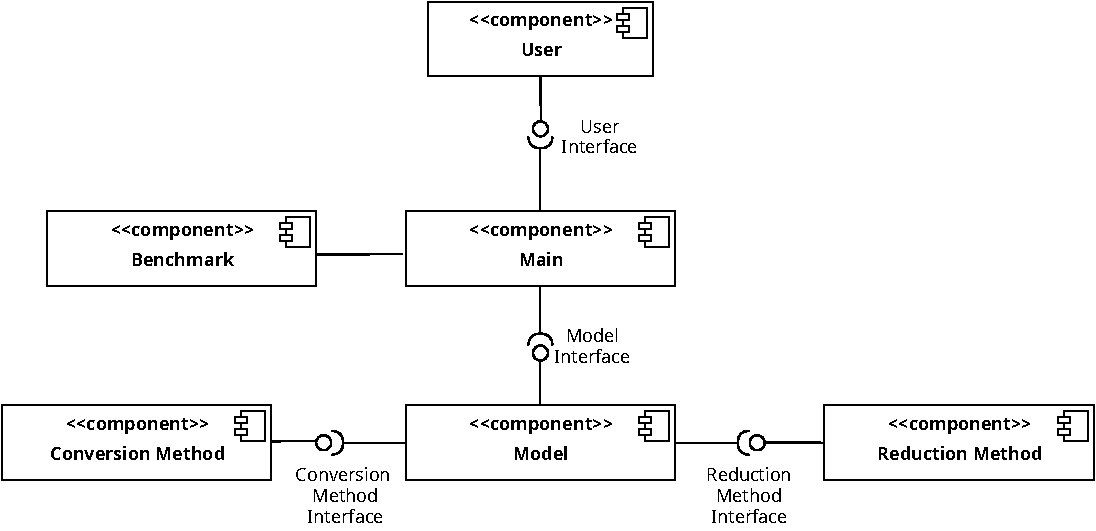
\includegraphics[keepaspectratio, width=0.8\textwidth]{img/components.pdf}
			\end{center}

			
			
		\subsection{Subsystem decomposition}
			\paragraph{Main Module}
                The main module is the main entry point of the process, responsible for executing the user interface, the algorithms and utilities from the model specific modules, the conversions, as well as dealing with benchmark flows and loading the necessary examples. There are two mandatory basic control flows and one optional one that depends on the theoretical feasibility that is to be proven: 
                \begin{enumerate}
                    \item Standard model reduction for a single model with user specified input
                    \item Benchmark flow using the provided examples, resulting in two sequential model reduction executions. They can not be parallelized, as they would infere with the caches and slow each other down. After the execution it converts one instance to the other model preserving model complexity or checks if they are equivalent.
                \end{enumerate}


			\paragraph{User Interface}
				The User Interface let's the user control the main module, provides means of input to the main module and displays the output from the main module. Also contains usage information. \\
				A text-based user interface is to be implemented (also called command-line interface). The user interface must contain a menu letting the user specify what control flow is to be executed, thus what task the user wants to perform. It must be able to either read the data from file or from the standard input of the terminal and display the input, output and summary on the standard output of the terminal, aswell as possible errors. \\
				The UserInterface provides functionality to control the program and to deliver outputs to the user. Therefore most functions are parameterless and take their input from the user, so those must ensure the validity of the user input. The only special case is the actual input data which is validated by a model specific function and the output functions which do not take user input. \\
\begin{verbatim}
Interface UserInterface {
    public Task select_task() {
        ensure Task exists
    }

    public ModelInterface select_model() {
        ensure model exists
    }
    
    public ReductionMethodInterface select_method(ModelInterface model) {
        require model not null
        ensure method exists && method compatible to model
    }
    
    public IOMethod select_input_method() {
        ensure input method exists
    }
    
    public FILE* file_input() {
        ensure file exists && file is closed after read
    }
    
    public char* stdin_input() {
        require limited input
        ensure input is read completely or rejected
    }
    
    public IOMethod select_output_method() {
        ensure output method exists
    }
    
    public FILE* set_output_location() {
        ensure file exists or create new file && containing directory exists
    }
    
    public void display_exec_file(FILE* output_destination) {
        require output_destination not null
        assure file is closed after write
    }
    
    public void display_exec_stdout(char* output) {
        require output not null && output limited
        ensure output is less than default terminal buffer size || output is paged
    }
}
\end{verbatim}				
			
			\paragraph{Model Interface}
                The model interface specifies the details of a model including the representation format, input validation functionality, concrete instances will hold an array of function pointers of the reduction method interface type for the concrete model. Depending on the task that the user wants to perform either one or another instance is used to execute the control flow. The data flow from the user via the main module is passed to the model interface instance which does the actual processing using the defined functions and one of the functions from the array holding the model reduction method pointers. Instances of this interface must also specify how to summarize and compute statistics over the result, i.e. the differences in the model and in model complexity. To be implemented are instances for DEs and WAs.
\begin{verbatim}
 Interface ModelInterface {
    ModelRepresentation representation require not null
    ReductionInterface*[] ReductionMethodInterface[]
    ConversionMethodInterface*[] conversions
    
    public ModelRepresentation validate_model_instance(char* input) {
        require input not null
        ensure model is valid wrt. representation
        
    }

    public char* summarize_reduction(ModelRepresentation input, ModelRepresentation reduced) {
        require input not null && reduced not null
    }
 }
\end{verbatim}

            \paragraph{Model Representation Interface}
                As the data needs to be validated, this interface shall specify a structure for holding an instance of the model.
\begin{verbatim}
 Interface ModelRepresentationInterface {
    struct ModelRepresentation require not null
 }
\end{verbatim}

			
			\paragraph{Reduction Method Interface}
                This interface is used to implement concrete reduction methods for a specific model. For each models there may be multiple reduction methods. To be implemented are the reduction methods specified in~\autocite{Cardelli2017MaximalAO, Kiefer2013OnTC}. 
\begin{verbatim}
 Interface ReductionMethodInterface {
    public ModelRepresentation reduce(ModelRepresentation input) {
        require input not null
        ensure return value valid and not null
    }
 }
\end{verbatim}

			
			\paragraph{Conversion/Equivalence Interface}
                Using the model interfaces, implementations of this interface shall provide a method to convert an instance of a model to another model or to prove the equivalence of two instances of different models. As of now this is a question to be further investigated in terms of theory. One open question is if there exists an isomorphism between the to be implemented methods and if so how to do the conversion or equivalence check without also transforming the model complexity (e.g. from DEs to WAs, how not to produce more or less states than there are implicitly in the DE representation). The interface should optimally provide methods for conversion in both direction, i.e. a programatically equivalence proof and shall be attached to both models that it converts as pointer.
\begin{verbatim}
 Interface ModelConversionInterface {
    public ModelRepresentation convert_left_to_right(ModelRepresentation left) {
        require left not null
        ensure output is valid in rights's representation
    }
    
    ModelRepresentation convert_right_to_left(ModelRepresentation right) {
        require right not null
        ensure output is valid in left's representation
    }
 }
\end{verbatim}

                
            \begin{center}
            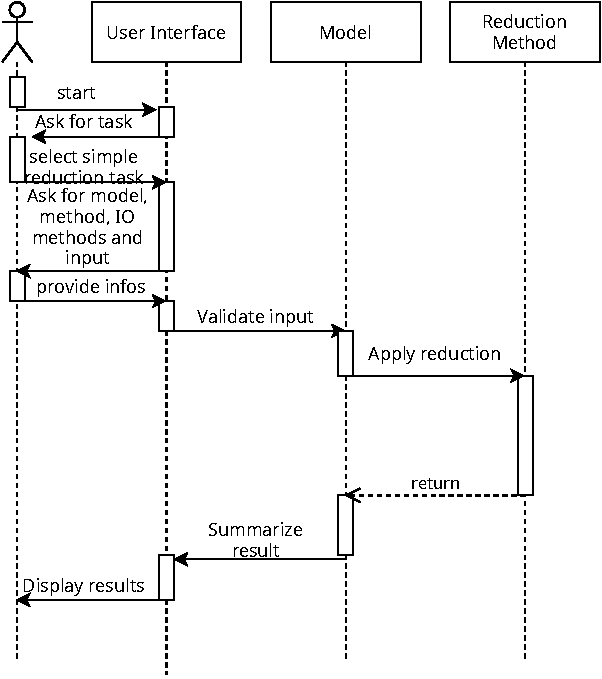
\includegraphics[keepaspectratio, width=0.5\textwidth]{img/sequence_simple.pdf} \\
            \noindent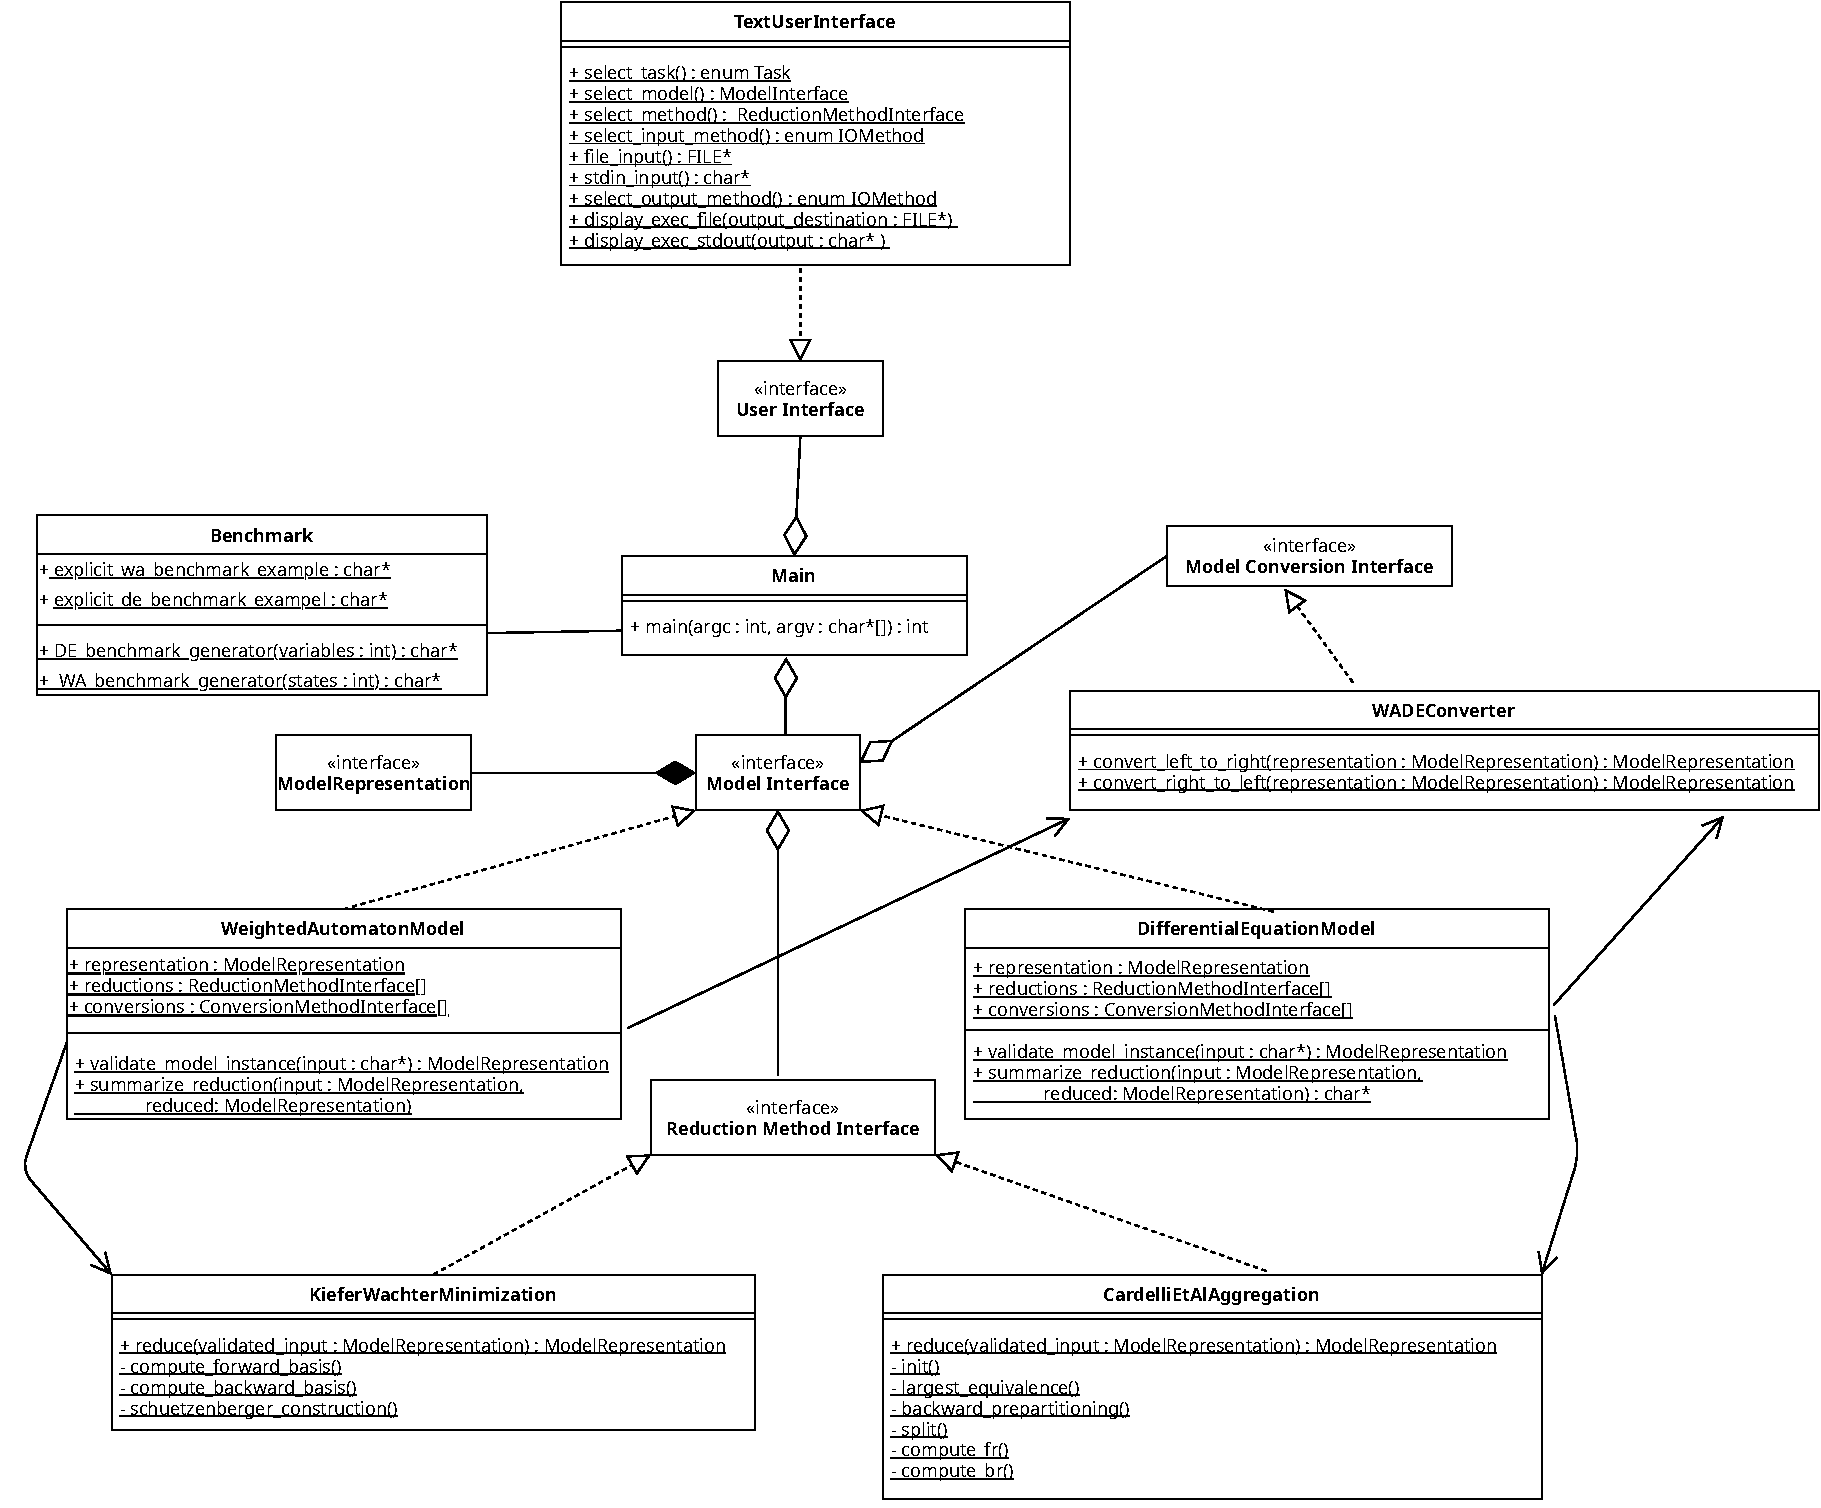
\includegraphics[keepaspectratio, width=1.1\textwidth]{img/class.pdf}
            
            \end{center}
